% (Written responses must be typeset and in pdf. Only one member of the group
% (should submit to the appropriate dropbox on Learn.)

% Due Wed, June 18, 11:59:59 PM

\documentclass[a4paper]{article}

\usepackage[english]{babel}
\usepackage[utf8]{inputenc}
\usepackage{amsmath}
\usepackage{graphicx}
\usepackage{parskip}
\usepackage{amssymb}
\usepackage{mathtools}
\usepackage{svg}
\usepackage{pdfpages}

\DeclarePairedDelimiter\ceil{\lceil}{\rceil}
\DeclarePairedDelimiter\floor{\lfloor}{\rfloor}

\title{ECE457A Assignment 2}
\author{
  Group 27 \\
  \\
  Lucas Wojciechowksi, Ariel Weingarten, Alexander Maguire, \\
  Austin Dobrik, Dane Carr}
\date{\today}

\begin{document}

\maketitle

\section{Question 1}

\subsection{Part A}

\subsubsection{Solution Representation}

Solutions will be represented as a set of $m$ vectors of varying length $l_{i}$ s.t. $\sum_{i=0}^{m}dim(v_{i}) = c$.
Each vector represents the route for one vehicle, and each element represents a city along the vehicle's route with cities being visited in order.

$v_{0} = \begin{bmatrix}
v_{0,0} & v_{0,1} & \cdots & v_{0,l_{0}}
\end{bmatrix} \\
v_{1} = \begin{bmatrix}
v_{1,0} & v_{1,1} & \cdots & v_{1,l_{1}}
\end{bmatrix} \\
\vdots \\
v_{m} = \begin{bmatrix}
v_{m,0} & v_{m,1} & \cdots & v_{m,l_{m}}
\end{bmatrix}$

\subsubsection{Neighbourhood Operators}

There will be two neighbourhood operators, one to change the order of the cities and one to change the length of a route.  The first operation is
to swap any two elements.  The elements can either be in the same vehicle vector, or in two different vehicle vectors.  The second operation is to
remove one element from a vehicle vector and add it to another.

\subsubsection{Objective Function}

Let $Depot_{c_{i}}$ be the distance between the depot and city $i$ \\
Let $D_{c_{i},c_{j}}$ be the distance between city $i$ and city $j$ \\
Let $S_{c_{i}}$ be the time required to service city $i$ \\

$\sum_{i=0}^{m}(Depot_{v_{i,0}} + Depot_{v_{i,l_{i}}} + \sum_{j=0}^{l_{i}-1}D_{v_{i,j},v_{i,j+1}} + \sum_{j=0}^{l_{i}}S_{v_{i,j}})$

\subsection{Part B}

To account for a constraint on the length of each route, we could penalize each solution that contains a route longer than $T$.  Every route that exceeds $T$ would add an additional cost $P$ to the objective function.  This way the SA algorithm would be able to probabilistically choose this poor solution if it needed to diversify.  The new objective function would be

$\sum_{i=0}^{m}(Depot_{v_{i,0}} + Depot_{v_{i,l_{i}}} + \sum_{j=0}^{l_{i}-1}D_{v_{i,j},v_{i,j+1}} + \sum_{j=0}^{l_{i}}S_{v_{i,j}} + \left.P\right|_{if cost(v_{i}) > T}^{})$

\section{Question 2}

% An industrial communication company is planning to lay cables to a new factory
% allowing all the factory’s units to be linked for the interchange of data. If
% it is constrained to bury the cable only along certain paths, then there would
% be an undirected graph representing which points are connected by those paths.
% Some of those paths might be more expensive, because they are longer, or
% require the cable to be buried deeper; these paths would be represented by
% edges with larger weights. For example, Figure 1 shows 5 factory’s units and
% the possible paths along which the cables can be buried.

% The minimum spanning tree (MST) of the graph that represents the factory’s
% units and paths can be used to decide the most cost-effective paths for laying
% cables. MST is a tree that spans all the nodes of the graph with a minimum
% cost. MST is widely used in different applications such as communication
% network, transportation networks, scheduling and data clustering. Different
% greedy algorithms have been proposed for finding a MST such as Prim-Jarnik,
% Kruskal’s and Baruvka’s Algorithms.

% In this problem, a MATLAB code that implements the Tabu Search algorithm for
% finding the MST of an undirected graph is given.

% - You should run each experiment several times and report the average results.

% - Units100.mat contains a sparse matrix Graph that represents the possible
%   paths between 100 factory’s units through which communication cables can be
%   laid. The element Graph (a, b) represents that cost of the path between
%   units a and b.

\subsection{Part A}

% a) Use the given functions to find the most cost-effective paths for the graph
% given in Units100.mat and report the total cost of laying the cables.

Using Kruskal's Algorithm, we calculate the most cost-effective paths for the
graph given in \texttt{Units100.mat} and find the cost of this solution to be
109.

\subsection{Part B}

% b) Run the code with different tabu list lengths (5, 10, 15, 25, 50) and
% report the cost obtained in each case. What do you observe?

Since the number of iterations was not specified, we have included a graph of the solution provided by the algorithm for iterations 1 through 100, averaged over 5 runs.

We observe that regardless of tabu length, all answers converge to the ideal answer of 109 around 90 iterations.

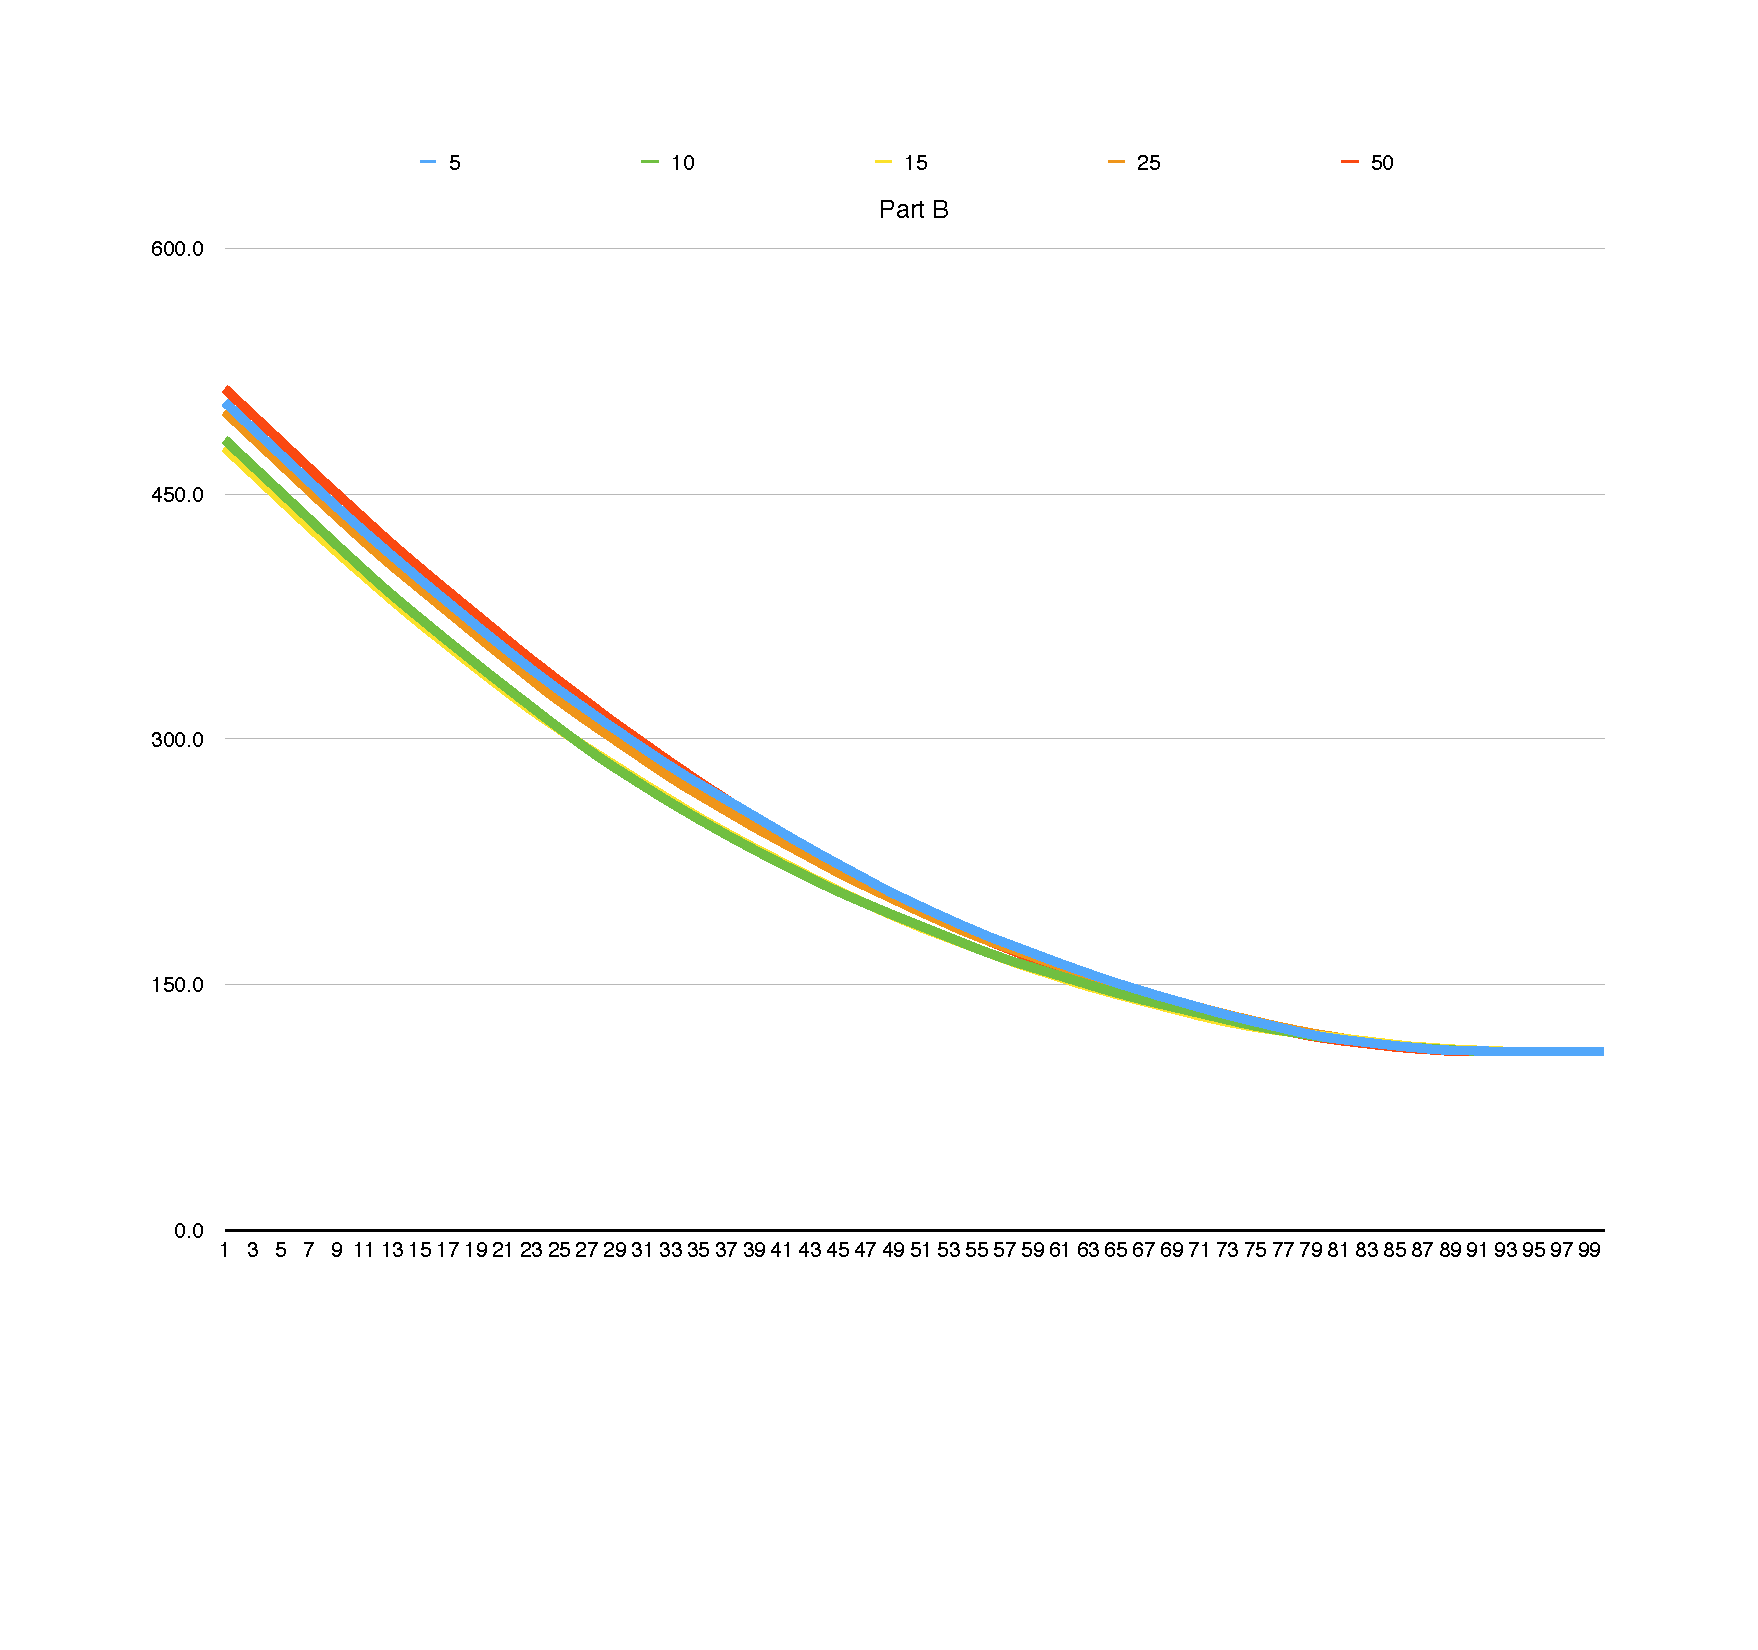
\includepdf[pages={1}]{q2/ab.pdf}

\subsection{Part C}

% Modify GetBestNeighbourST.m and other necessary functions to include the use
% of an aspiration criterion. The aspiration criterion in this problem could be
% to allow solutions that are better than the currently known best solution.
% Repeat (a) and (b) with the modified code.

We modified \texttt{GetBestNeighbourST.m}'s use of the tabu list to implement an aspiration criterion. In particular, we changed

\begin{verbatim}
    % 2. Check if the edge to be removed (e1) is in the tabu list
    if TabuEdges(NT1(e1), NT2(e1)) == 0
        if NewSTCost < BestNeighbourSTCost
            BestNeighbourST = NewST;
            BestNeighbourSTCost = NewSTCost;

            TabuEdgeN1 = N1(BestEdge);
            TabuEdgeN2 = N2(BestEdge);
            AddTabuMove = true;
        end
    end
\end{verbatim}

to read

\begin{verbatim}
    % 2. Check if the edge to be removed (e1) is in the tabu list
    if (TabuEdges(NT1(e1), NT2(e1)) == 0 && NewSTCost < BestNeighbourSTCost) || ...
                (TabuEdges(NT1(e1), NT2(e1)) ~= 0 && NewSTCost < STCost)

            BestNeighbourST = NewST;
            BestNeighbourSTCost = NewSTCost;

            TabuEdgeN1 = N1(BestEdge);
            TabuEdgeN2 = N2(BestEdge);
            AddTabuMove = true;
        end
    end
\end{verbatim}

We graphed this code in the same way as part B. Note that the graph is shallower as all runs converge to the ideal answer more quickly than in part A.

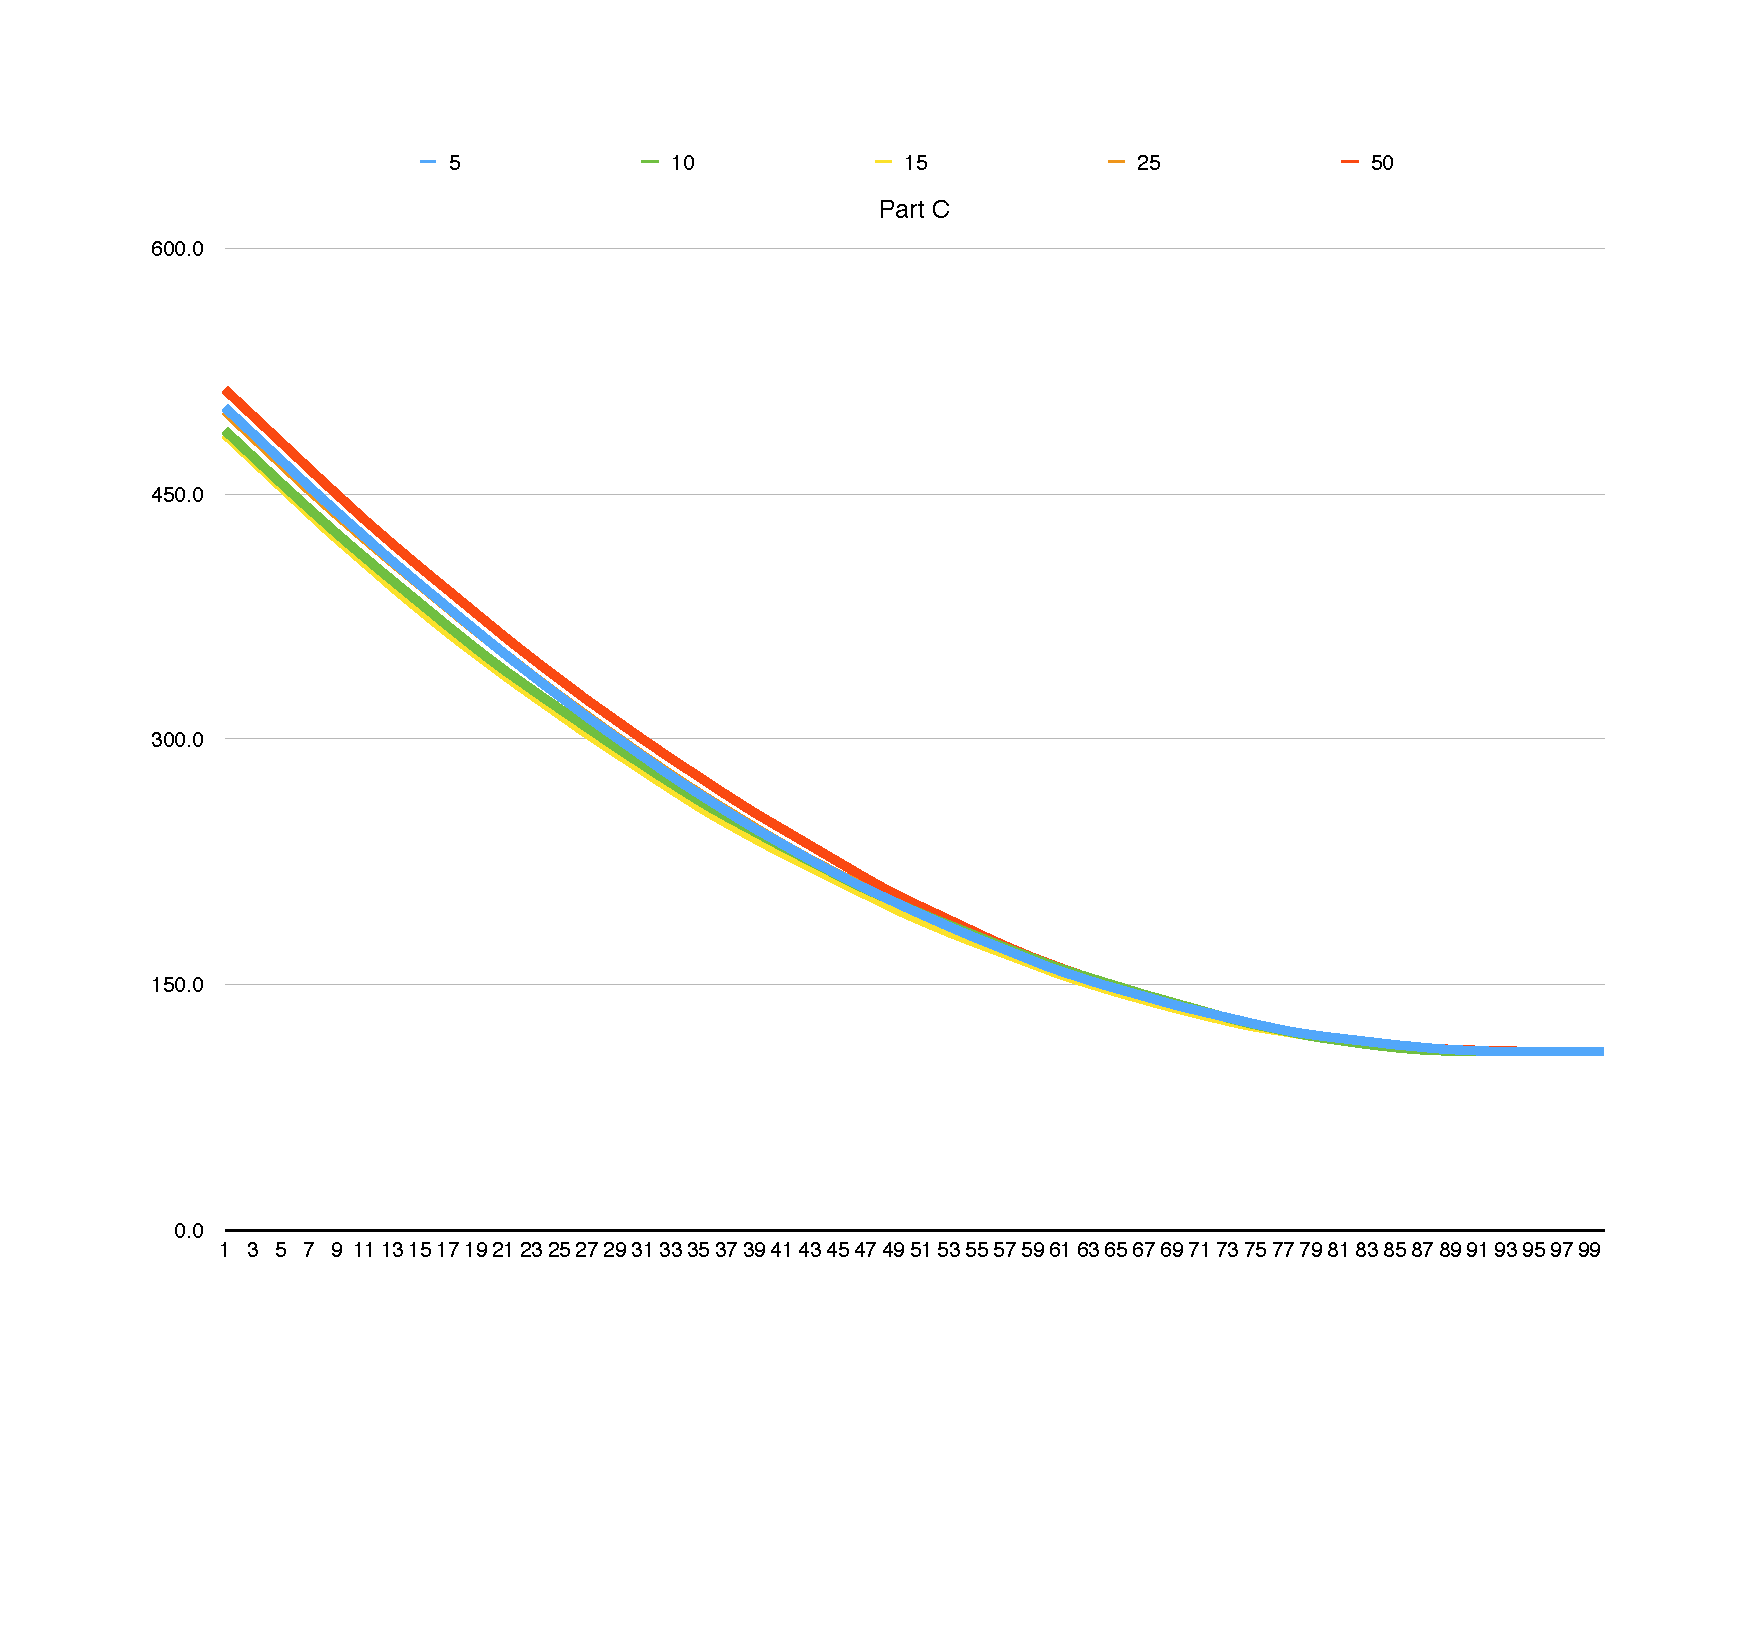
\includepdf[pages={1}]{q2/c.pdf}

\subsection{Part D}

% Suppose that splitters need be used at the factory’s units if the number of
% cables going through the unit exceeds 2. The cost of the splitter increases as
% the number of cables connected to the splitter n increases and it can be
% calculated as (omitted) Modify GetBestNeighbourST.m and other necessary
% functions to consider adding the cost of the splitters. Repeat (a) and (b)
% with the modified code.

In this part, we replaced all cost calculations with a call to the function
\begin{verbatim}
function Cost = GetCost(Graph, ST)

EdgeCost = sum(sum(Graph .* ST)) / 2;
NodeCost = sum(10 ./ (1 + exp(-1 * sum(Graph) ./ 10)));

Cost = EdgeCost + NodeCost;
\end{verbatim}

This new cost function did not produce an ideal solution with Kruskal's algorithm.

Using Tabu Search, however, it did converge to an answer at a cost of 1103. We graphed the solution versus iterations averaged over 5 runs in the same way as part A.
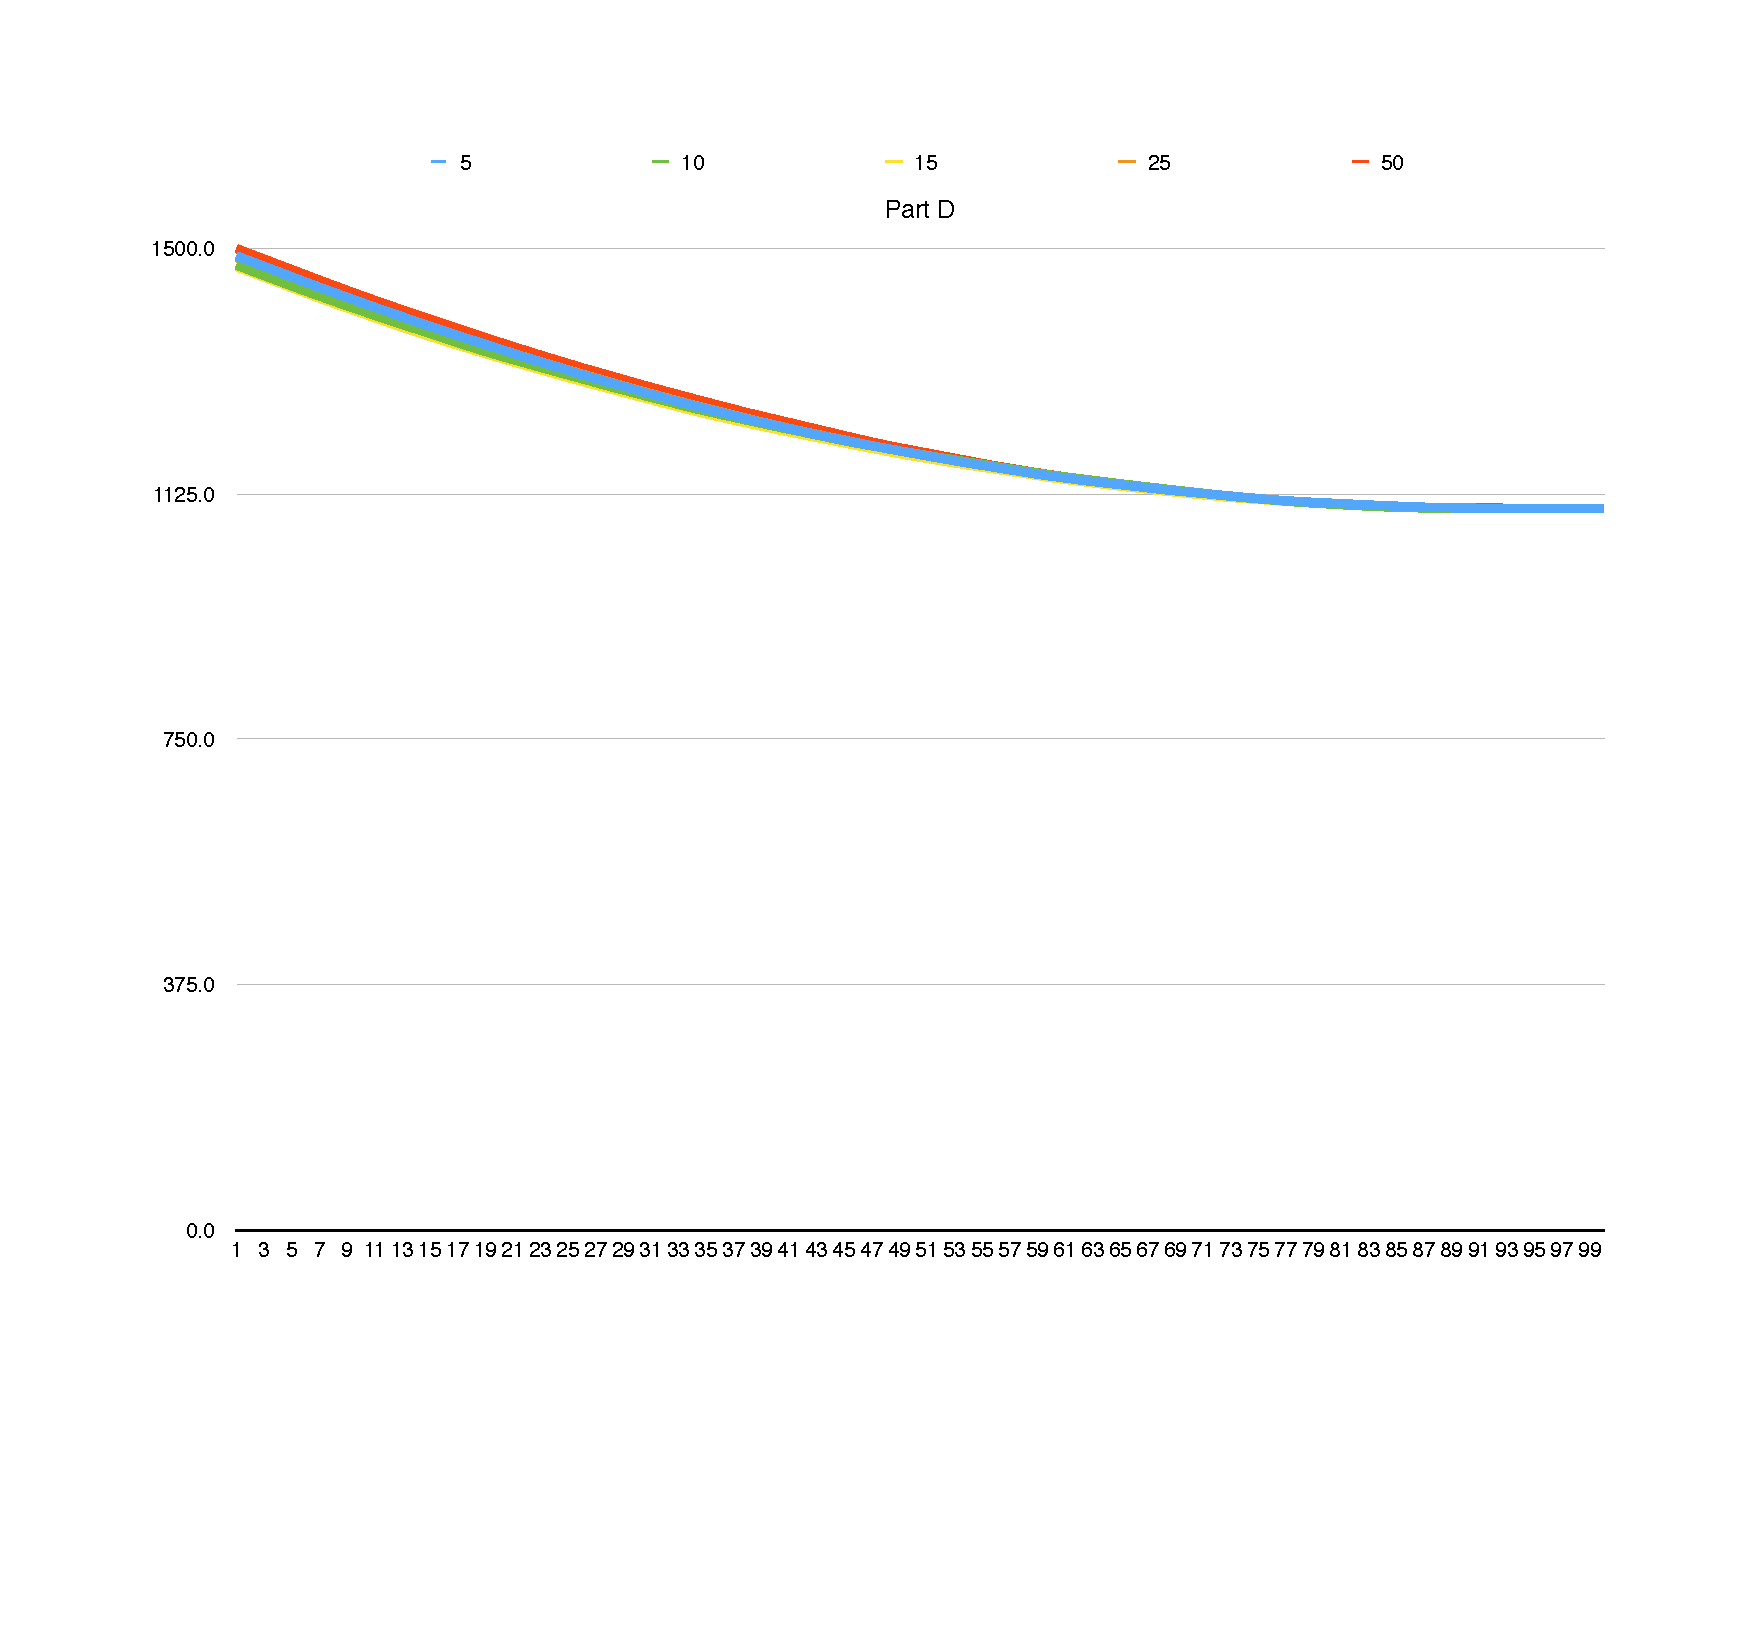
\includepdf[pages={1}]{q2/d.pdf}

We also tried using the improvements from part C in the new problem proposed for part D and found it to have better performance characteristics again. We graphed the solution versus iterations averaged over 5 runs in the same way as part A.

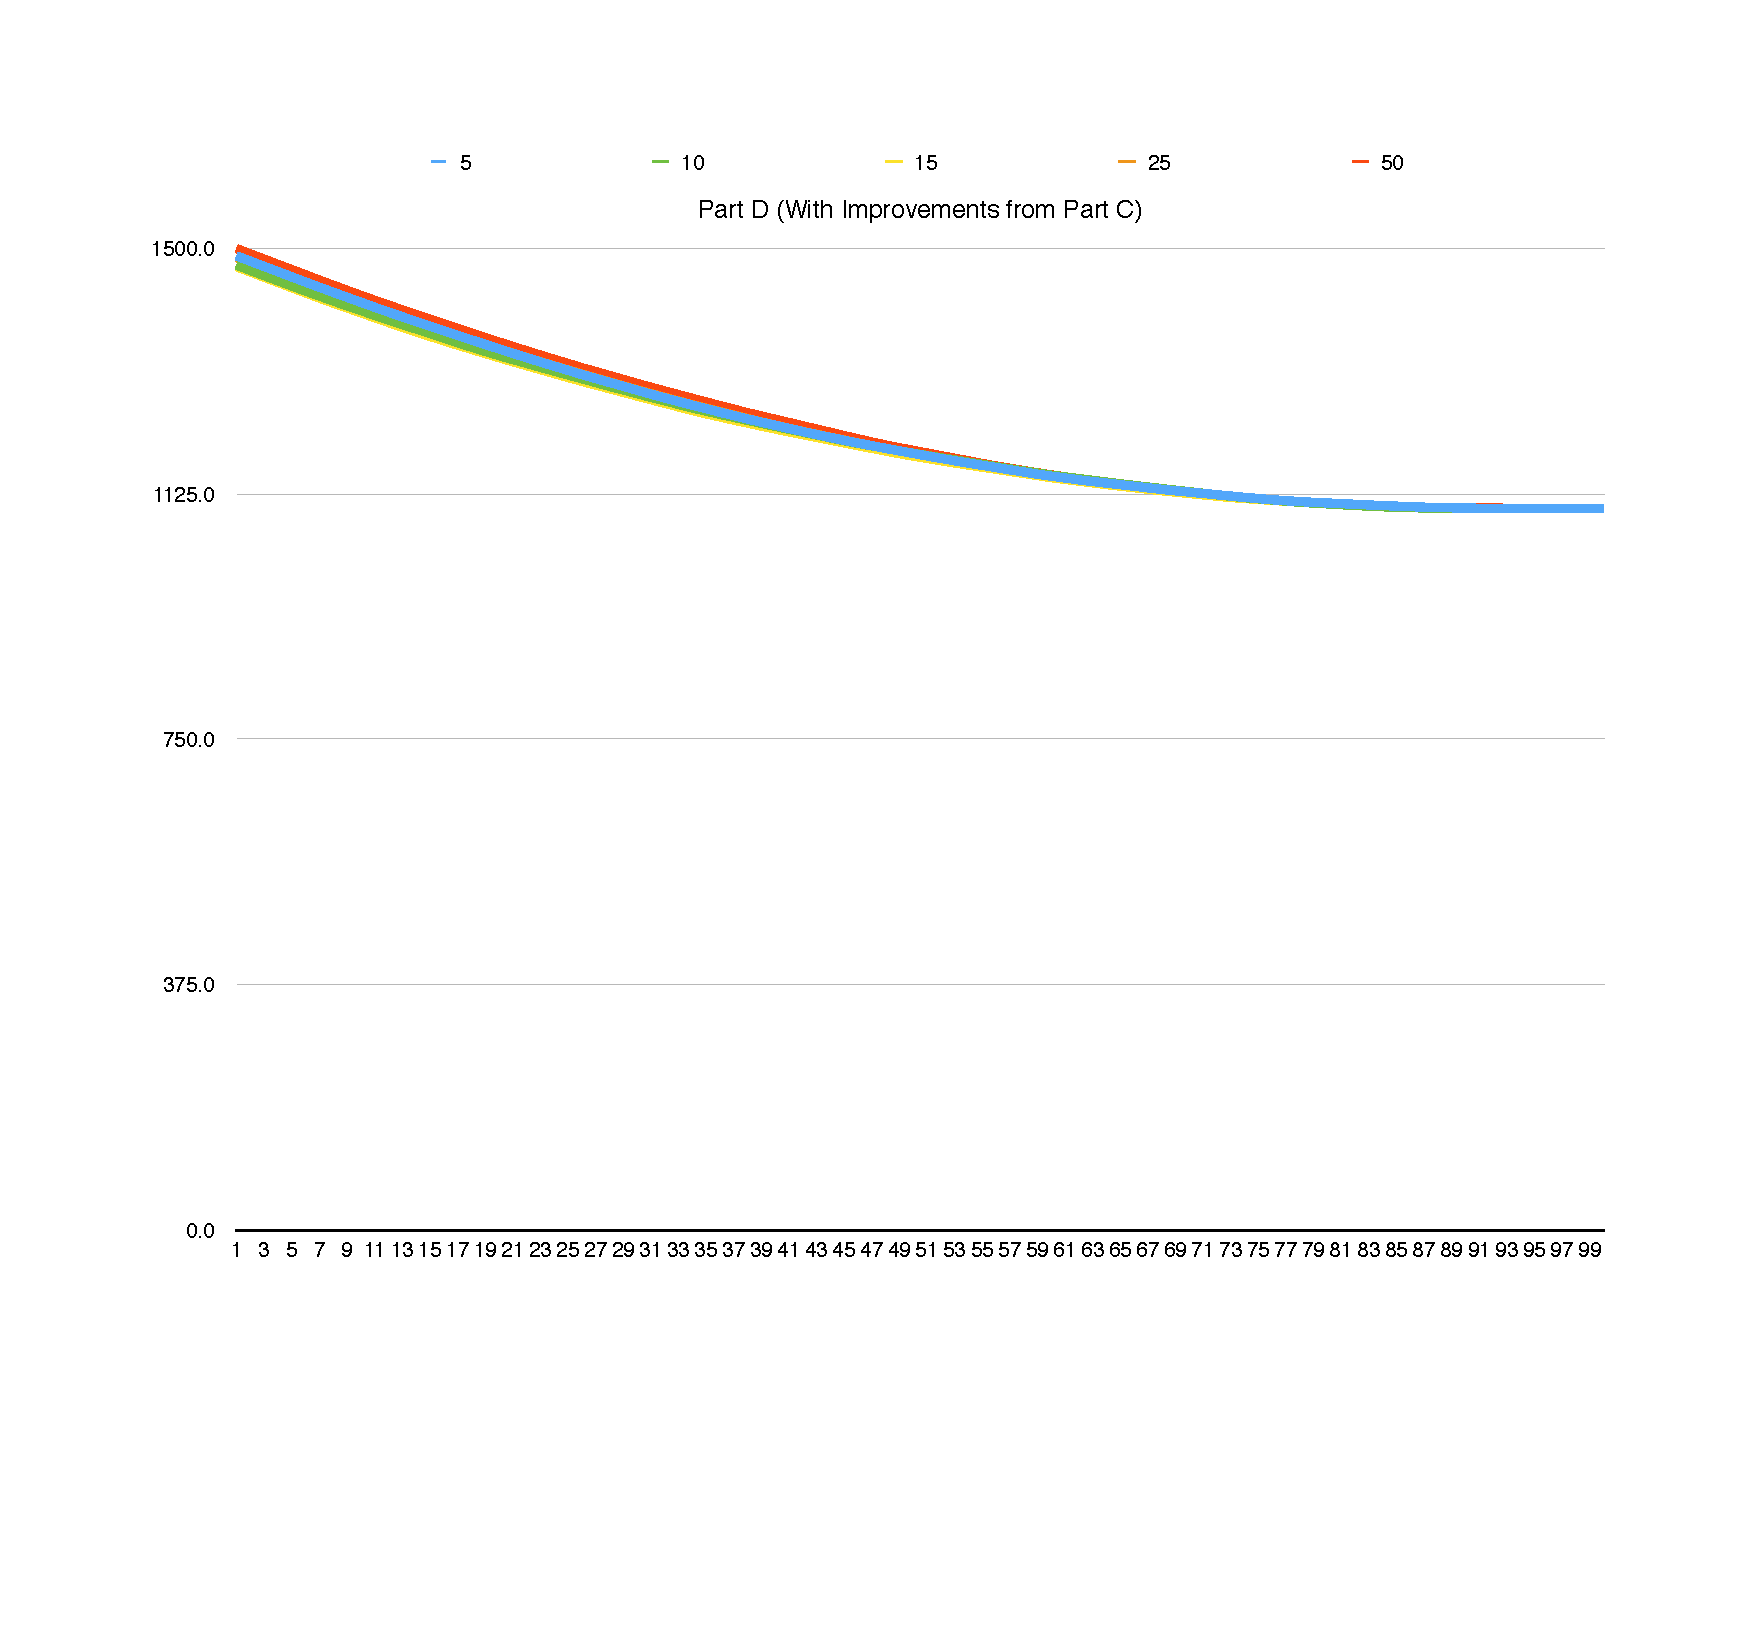
\includepdf[pages={1}]{q2/dc.pdf}

\subsection{Part E}

% Compare between Tabu Search and the greedy algorithm of Kruskal as an example
% for greedy algorithms.

In parts A and B, Kurskal's algorithm produced the same answer as Tabu Search in many orders of magnitude less time. However, in part D, the nature of the problem changed such that a greedy algorithm such as Kurskal's was no longer suitable.

In general, for problems like this, one should use a greedy algorithm if at all feasible; the greedy algorithm will produce a guaranteed optimal solution in $O(n)$ time. However, when a greedy algorithm is not feasible, such with the complex cost function in part D, a Tabu Search algorithm is a good tool to try.

\end{document}
